%------------------------------------------------------------------------------
\chapter{Modified Format}
\label{sec:app_2}
%------------------------------------------------------------------------------
\begin{figure}[h!]
\centering
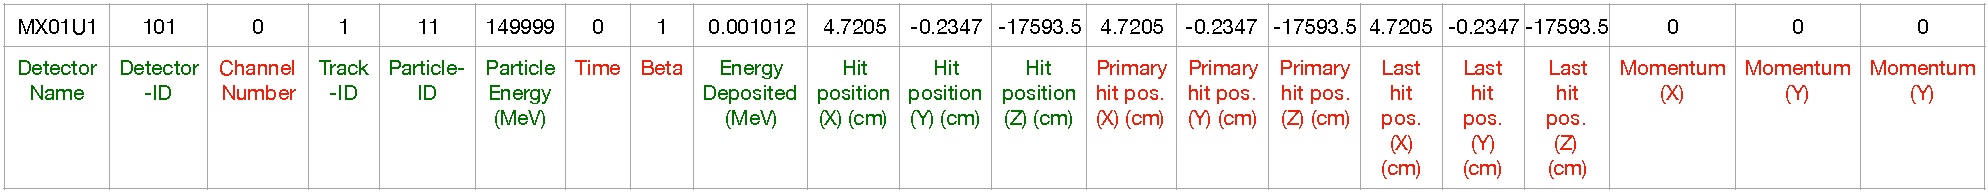
\includegraphics[width=18cm]{thesis_figures/TGEANT_format.pdf}
\caption{Snippet of the format fed to CORAL}
\label{fig:Format}
\end{figure}

The above figure is a snippet of the modified format which was fed to CORAL for the tracking detector. The line in black is the part which was actually fed to CORAL in a compressed plain text format. The second line in the figure gives a description about the values. The green colour is an indication that the information was available in the output of the simulation while the ones in red were not available and were substituted by some reasonable values. As it can be seen in the figure each plane of the tracking detector is fed individually. For CORAL, the planes were exactly replicated with a shifted z position for each hit. 
The format for the calorimeters is exactly the same with only the information about the detector name, detector-ID and energy deposited available from the original simulation while the rest is replaced with zero.
